% !Mode:: "TeX:UTF-8"
% !TEX program  = xelatex
\documentclass[a4paper]{article}
\usepackage{amsmath}
\usepackage{amssymb}
\usepackage{ctex}
\usepackage{graphicx}
%\usepackage{braket}
\usepackage[european]{circuitikz}
\usepackage{multirow}
\usepackage{geometry}
\usepackage{cite}
\geometry{left=2.5cm,right=2.5cm,bottom=2.5cm,top=2.5cm}
\title{物理化学实验17:BZ振荡反应}
\author{薛明怡\quad 151250177\quad 化学化工学院}
\date{\today}
\begin{document}
\maketitle
%%\tableofcontents
\bibliographystyle{unsrt}
\section{实验目的}
\begin{enumerate}
\item 了解自然界中存在的非平衡非线性现象.
\item 掌握求Belousov-Zhabotinsli反应(BZ振荡反应)活化能的实验方法.
\item 通过``翻转课堂''的实施, 培养自主创新意识.
\end{enumerate}
\section{实验原理}
\subsection{非平衡态热力学}
经典热力学三大定律:(适用条件: 封闭系统, 平衡态, 不做非体积功)
\begin{enumerate}
	\item \textbf{第一定律} $\Delta U=Q+W$
	\item \textbf{第二定律} $dS\ge \frac{\delta Q}{T}$
	\item \textbf{第三定律} $\lim_{T \to 0}S=0$ (完美晶体)
\end{enumerate}	
\par
根据热力学第二定律, 在孤立体系中, 
自发变化的方向由有序到无序, 混乱度增加,趋向于平衡态. 
而自然界中广泛存在的有序形貌促进了20世纪50年代非平衡热力学研究的发展.

\subsection{耗散结构}
热力学系统可以分为三类, 热力学三大定律适用的平衡态系统, 
局域平衡假设适用的近平衡态系统(线性非平衡态), 
以及远平衡态系统(非线性非平衡态系统).\par
耗散结构是指非线性非平衡态系统由于本身的非线性动力学机制
而有可能产生宏观时空有序的结构.\par
本实验研究的BZ振荡反应是一种典型的耗散结构.
\subsection{BZ振荡}
由溴酸盐, 有机物在酸性介质中, 在有(或无)金属离子催化剂催化下, 
某些中间组分的浓度发生\textbf{周期性变化}, 溶液颜色出现交替变化的现象, 即发生化学振荡.
化学振荡反应的必要条件之一是该反应必须是自催化反应. 化学振荡现象的发生必须满足如下几个条件:
\begin{enumerate}
    \item 反应必须是敞开体系且远离平衡态, 即$\Delta_{r} G_{m}$为较负的值.
    \item 反应历程中应包含自催化的步骤.
    \item 体系中必须能有两个准定态(稳态)存在.
\end{enumerate}
\subsection{自催化反应}
在给定条件下的反应体系, 反应开始后逐渐形成并积累了某种产物或中间体, 这些产物具有催化功能, 
使反应经过一段诱导期后出现大大加速的现象, 这种作用称为自(动)催化作用. 其特征之一是存在着初始的诱导期. 
大多数自动氧化过程都存在自催化作用. 油脂腐败, 橡胶变质以及塑料制品的老化均属于包含链反应的自动氧化过程, 
反应开始进行很慢, 但都被其所产生的自由基所加速.
\textbf{马洛卡模型}
$1$分子A自身分解产生$1$分子B和$1$分子C, 其中B可以迅速与A结合生成络合物AB, 该络合物又继续分解, 
生成$2$分子B和$1$分子C. 生成物B参与第二步反应和第三步反应, 充当了反应的催化剂, 
因此该反应被成为自催化反应. 反应历程如下:
\begin{equation}
	\begin{aligned}
		&A \stackrel{k_{1}}{\longrightarrow} B + C\\
		&A + B \stackrel{k_{2}}{\longrightarrow} AB\\
		&AB \stackrel{k_{3}}{\longrightarrow} B + C\\
	\end{aligned}
\end{equation}
\par
在常规反应中, 反应速率与反应物浓度相关:
\begin{equation}
r \propto [A]^{n}\\
\end{equation}
\par
因此, 随着反应的进行, 反应物浓度降低, 反应速率减缓.\par
而在自催化反应中, 一开始反应历程遵循上述表达式, 但随着反应的进行, 
反应历程发生变化, 虽然反应物浓度降低, 
但是自催化剂浓度增加对反应速率的贡献超过了反应物浓度降低对反应速率的减缓效应.\\
\begin{equation}
r \propto [A]^{x}[B]^{y}\\
\end{equation}
\begin{figure}[!h]
	\centering
	\includegraphics[width=0.30\paperwidth]{fig/mechanics.png}\\
	\caption{反应机理}\label{wf}
\end{figure}
\subsection{FKN机理}
以本实验为例, 原料溴酸钾, 丙二酸, 硫酸铈铵, 硫酸, 反应生成溴离子,
次溴酸, 亚溴酸, 二氧化溴, 丙二酸溴, 单质溴等中间产物, 
涉及二十几个基元反应.\par
主要基元反应可以被分为三组,
\begin{enumerate}
	\item \textbf{A过程}
	\begin{enumerate}
		\item $BrO_{3}^{-} + Br^{-} + H^{+} \to HBrO_{2} + HOBr$ (控速步)
		\item $HBrO_{2} + Br^{-} + H^{+} \to 2HOBr$
		\item $HOBr + Br^{-} + H^{+} \to Br_{2} + H_{2}O$
		\item $Br_{2} + CH_{2}(COOH)_{2} 
				\to BrCH(COOH)_{2} + H^{+} + Br^{-}$
	\end{enumerate}
	\item \textbf{B过程}
	\begin{enumerate}
		\item $HBrO_{2} + BrO_{3}^{-} + H^{+}
				\to 2BrO_{2} + H_{2}O$
		\item $BrO_{2} + Ce^{3+} + H^{+}
				\to HBrO_{2} + Ce^{4+}$
		\item $2HBrO_{2}
				\to BrO_{3}^{-} + HOBr + H^{+}$
	\end{enumerate}
	\item \textbf{关联反应}
	\begin{enumerate}
		\item $4Ce^{4+} + BrCH(COOH)_{2} + H_{2}O + HOBr 
				\to 2Br^{-} + 4Ce^{3+} + 3CO_{2} + 6H^{+}$
		\item $2H^{+} + 2BrO_{3}^{-} + 3CH_{2}(COOH)_{2} 
				\to 2BrCH(COOH)_{2} + 3CO_{2} + 4H_{2}O$
	\end{enumerate}
	\item \textbf{总反应}
	\begin{enumerate}
		\item $2H^{+} + BrO_{3}^{-} + 2CH_{2}(COOH)_{2} 
				\to 2BrCH(COOH)_{2} + 3CO_{2} + 4H_{2}O$
	\end{enumerate}
\end{enumerate}
\par
当溴离子的浓度低于临界浓度时主要发生A过程, 
低于临界浓度时主要发生B过程. 其中临界浓度由反应式$A_{b}$和$B_{a}$平衡推导出, \\
\begin{equation}
	\begin{aligned}
			&[Br^{-}]_{crit} = \frac{k_{B_a}}{k_{A_b}}[BrO_{3}^{-}]\\
			&= 5\times 10^{-6} [BrO_{3}^{-}]\\
	\end{aligned}
\end{equation}

\subsection{检测手段}
在本实验中通过测量电势和观察颜色, 形成对耗散结构的时空有序性的一定认知.
\subsection{诱导期}
BZ振荡反应中诱导期与反应速率常数成反比, 测量一系列不同温度下的诱导期, 
再利用阿伦尼乌斯公式, 可以求出反应的活化能.\\
\begin{figure}[!h]
	\centering
	\includegraphics[width=0.30\paperwidth]{fig/time.png}\\
	\caption{自催化反应历程}\label{wf}
\end{figure}
\begin{equation}
	\begin{aligned}
		\frac{1}{t} &\propto k\\
		\ln{\frac{1}{t}} &= \ln{A} - (\frac{E_{a}}{R})\times \frac{1}{T}\\
	\end{aligned}
\end{equation}
\begin{figure}[!h]
	\centering
	\includegraphics[width=0.30\paperwidth]{fig/energy.png}\\
	\caption{计算活化能方法}\label{wf}
\end{figure}
\subsection{同心圆实验}
观察BZ振荡随空间的有序变化. 
\subsection{自主探索}
\begin{enumerate}
	\item 反应物浓度变化的影响
	\item 原料添加顺序的影响
	\item 恒温时间长短的影响
	\item 搅拌速率的影响
\end{enumerate}
\section{仪器与药品}
\begin{enumerate}
    \item \textbf{仪器:} 低温恒温槽, 带夹套恒温反应釜, 铂电极, 甘汞电极(以硫酸为液接),
		磁力搅拌机, 5mL移液枪, 数据采集接口装置, 电脑; 4只小烧杯, 5mL量筒, 2支玻棒, 1套培养皿, 洗耳球, 试管夹
    \item \textbf{药品:} 0.004mol/L硫酸铈铵溶液, 0.25mol/L溴酸钾溶液, 0.45mol/L丙二酸溶液, 3mol/L硫酸溶液
\end{enumerate}
\begin{figure}[!h]
	\centering
	\includegraphics[width=0.30\paperwidth]{fig/config.png}\\
	\caption{实验装置}\label{wf}
\end{figure}
\section{实验步骤}
\subsection{实验准备}
洗净培养皿, 漏斗, 烧杯, 置于$100^\circ$C烘箱中干燥.
\subsection{测量电势随时间变化}
将恒温槽设为$30^\circ$C.\par
取1支硫酸电极, 将1mol/L硫酸溶液从支管口加入电极, 用洗瓶将电极外壁擦干净, 
硫酸电极接入数据采集口负极, Pt电极接入正极. 清洗电极底部和反应釜, 用滤纸擦干. 
洗涤并擦干搅拌子, 放入反应釜中.\par
用移液枪分别移取5mL溴酸钾, 丙二酸和硫酸溶液到反应釜中, 将反应釜和电极盖拼装好, 
置于磁力搅拌机上, 调节转速为400r/min.\par
洗涤5mL量筒, 并用少量硫酸铈铵溶液润洗. 用移液枪移取5mL硫酸铈铵溶液到量筒中, 
用试管夹将量筒固定到恒温槽中恒温, 开始计时恒温5min.\par
在软件中设置X轴范围为$[0, 600]s$, Y轴范围为$[300, 1200]mV$. 点击开始, 观察基线电势. \par
取出$30^\circ$C的硫酸铈铵溶液, 从漏斗口导入反应釜, 此时将出现电势突跃. 
用洗耳球将漏斗中残余的反应液吹入反应釜. 经过一段时间后, 电势下降, 
待出现3个完整的波形后可停止程序并保存数据.\par
重复上述步骤, 测量$35^\circ$C, $40^\circ$C, $45^\circ$C, $50^\circ$C下的数据.
\subsection{同心圆实验}
分别在三个烘干的小烧杯a(较大), b, c中称取约0.5g溴酸钾, 0.05g溴化钾, 0.lg丙二酸.\par
向烧杯b和c中加入1mL去离子水, 搅拌使固体溶解.\par
向烧杯a中加入5mL去离子水, 1mL 3mol/L的硫酸溶液, 以较大的培养皿为水浴缸, 倒入开水, 
放入小烧杯a, 搅拌溶解.\par
将烧杯转入通风处中, 将b和c中溶液倒入烧杯a, 待溶液褪色后, 加入约1mL亚铁灵溶液, 搅拌并观察颜色变化.\par
将溶液倒进小培养皿并轻轻晃动铺开, 将大培养皿中的水倒尽擦干, 盖在小培养皿上, 观察颜色变化.
\subsection{收尾}
清洗整理仪器.
\section{拓展实验}
1. 停止磁子搅拌后的电势变化\par
2. 将稀释10倍的亚铁灵溶液代替硫酸铈铵溶液作为催化剂\par
3. 取$2.5mL$硫酸溶液稀释到$5mL$观察反应电势\par
反应定性结论及现象详见讨论部分和误差分析.
\section{数据处理}
\begin{figure}[!h]
	\centering
	\includegraphics[width=0.50\paperwidth]{fig/experiment.png}\\
	\caption{时间$\ln(\frac{1}{t})$对温度$\frac{1}{T}$作图}
\end{figure}
\par
用一次函数$Y = k\times X + b$按最小二乘法优化拟合参数如下,
\begin{equation}
	\begin{aligned}
		\ln A &= b = 14.50\\
		-\frac{E_{a}}{R} &= k = -6.092\times 10^{3}\\
		R^{2} &= \frac{SSR}{SST} = \frac{\sum{(\hat{y_{i}}-\bar{y})^{2}}}{\sum{(y_{i}-\bar{y})^{2}}}\\
					&=0.9904\\
	\end{aligned}
\end{equation}
\par
因此,
\begin{equation}
	\begin{aligned}
		Ea &= -R\times k\\
			 &= -8.314 \times (-6.092 \times 10^{3})\\
			 &= 50.65 kJ/mol\\
	\end{aligned}
\end{equation}
\newpage
\section{思考与讨论}
\begin{enumerate}
	\item 本实验记录的电动势主要代表什么?与能斯特方程求得的电势有什么不同?\\
	本实验记录的电势代表振荡过程的系统的综合电势,
	主要反映了反应过程中离子的浓度随着反应进程的变化, 
	是非平衡态的电势, 而Nernst方程求得的电位是平衡时的电势.
	\item 影响诱导期, 振荡周期, 振荡寿命的主要因素.
	\begin{itemize}
		\item 温度: 温度越高, 诱导期越短, 振荡周期越短.
		\item 催化剂: 催化离子可以影响反应速率.
		\item 溶液浓度: 根据速率方程, 溶液浓度越高, 反应速率越快.
		\item 溶液酸碱度: $H^{+}$浓度决定了两个稳态距离平衡态的远近. 
	\end{itemize}
	\item 自催化发生在哪一个过程? 自催化剂是何种物质?\\
	自催化剂为$Br^{-}$, 发生在A过程.
	\item 如何理解本实验为开放系统? 并且远离平衡态?\\
	系统与外部环境进行了物质和能量的交换, 
	并且采用了适当的有序结构来耗散环境传来的物质和能量.
	\item 两个稳态是哪两个状态?\\
	A过程与B过程时两个稳态, A过程中消耗$Br^{-}$, B过程中产生$Br^{-}$, 
	当$Br^{-}$浓度超过$Br^{-}_{crit}$时A过程占主导,
	否则B过程主导, 因此在两个状态间循环往复.
	\item 实验现象的观察和解释.\\
	在电势测量过程中, 体系中溶液颜色会产生黄色和无色的交替变化,
	电势高时为黄色, 电势低时为无色. 
	\item 同心圆的形成机制?\\
	BZ振荡反应的电势测定反映的是耗散体系在时间上的有序性,
	而同心圆实验反映的是耗散体系在空间上的有序性. 在
	$KBr -- KBrO_{3} -- H_{2}SO_{4}$系统中加入丙二酸和亚铁灵
	试剂, 假设体系有两个稳态A和B, 在静置条件下, 体系的某一点
	$Br^{-}$浓度大于临界值, 从而与周围的溶剂反应被消耗掉, 
	从而在这一点的溴离子浓度降低, 周围的离子浓度升高, 圆环向外扩展,
	形成红蓝相间的同心圆花纹. 以下两张图分别为反应开始和反应终了时的现象. 实验产生溴蒸气, 
	因此在实验结束时可以看到体系中产生的大量气泡.
	\begin{figure}[!h]
		\centering
		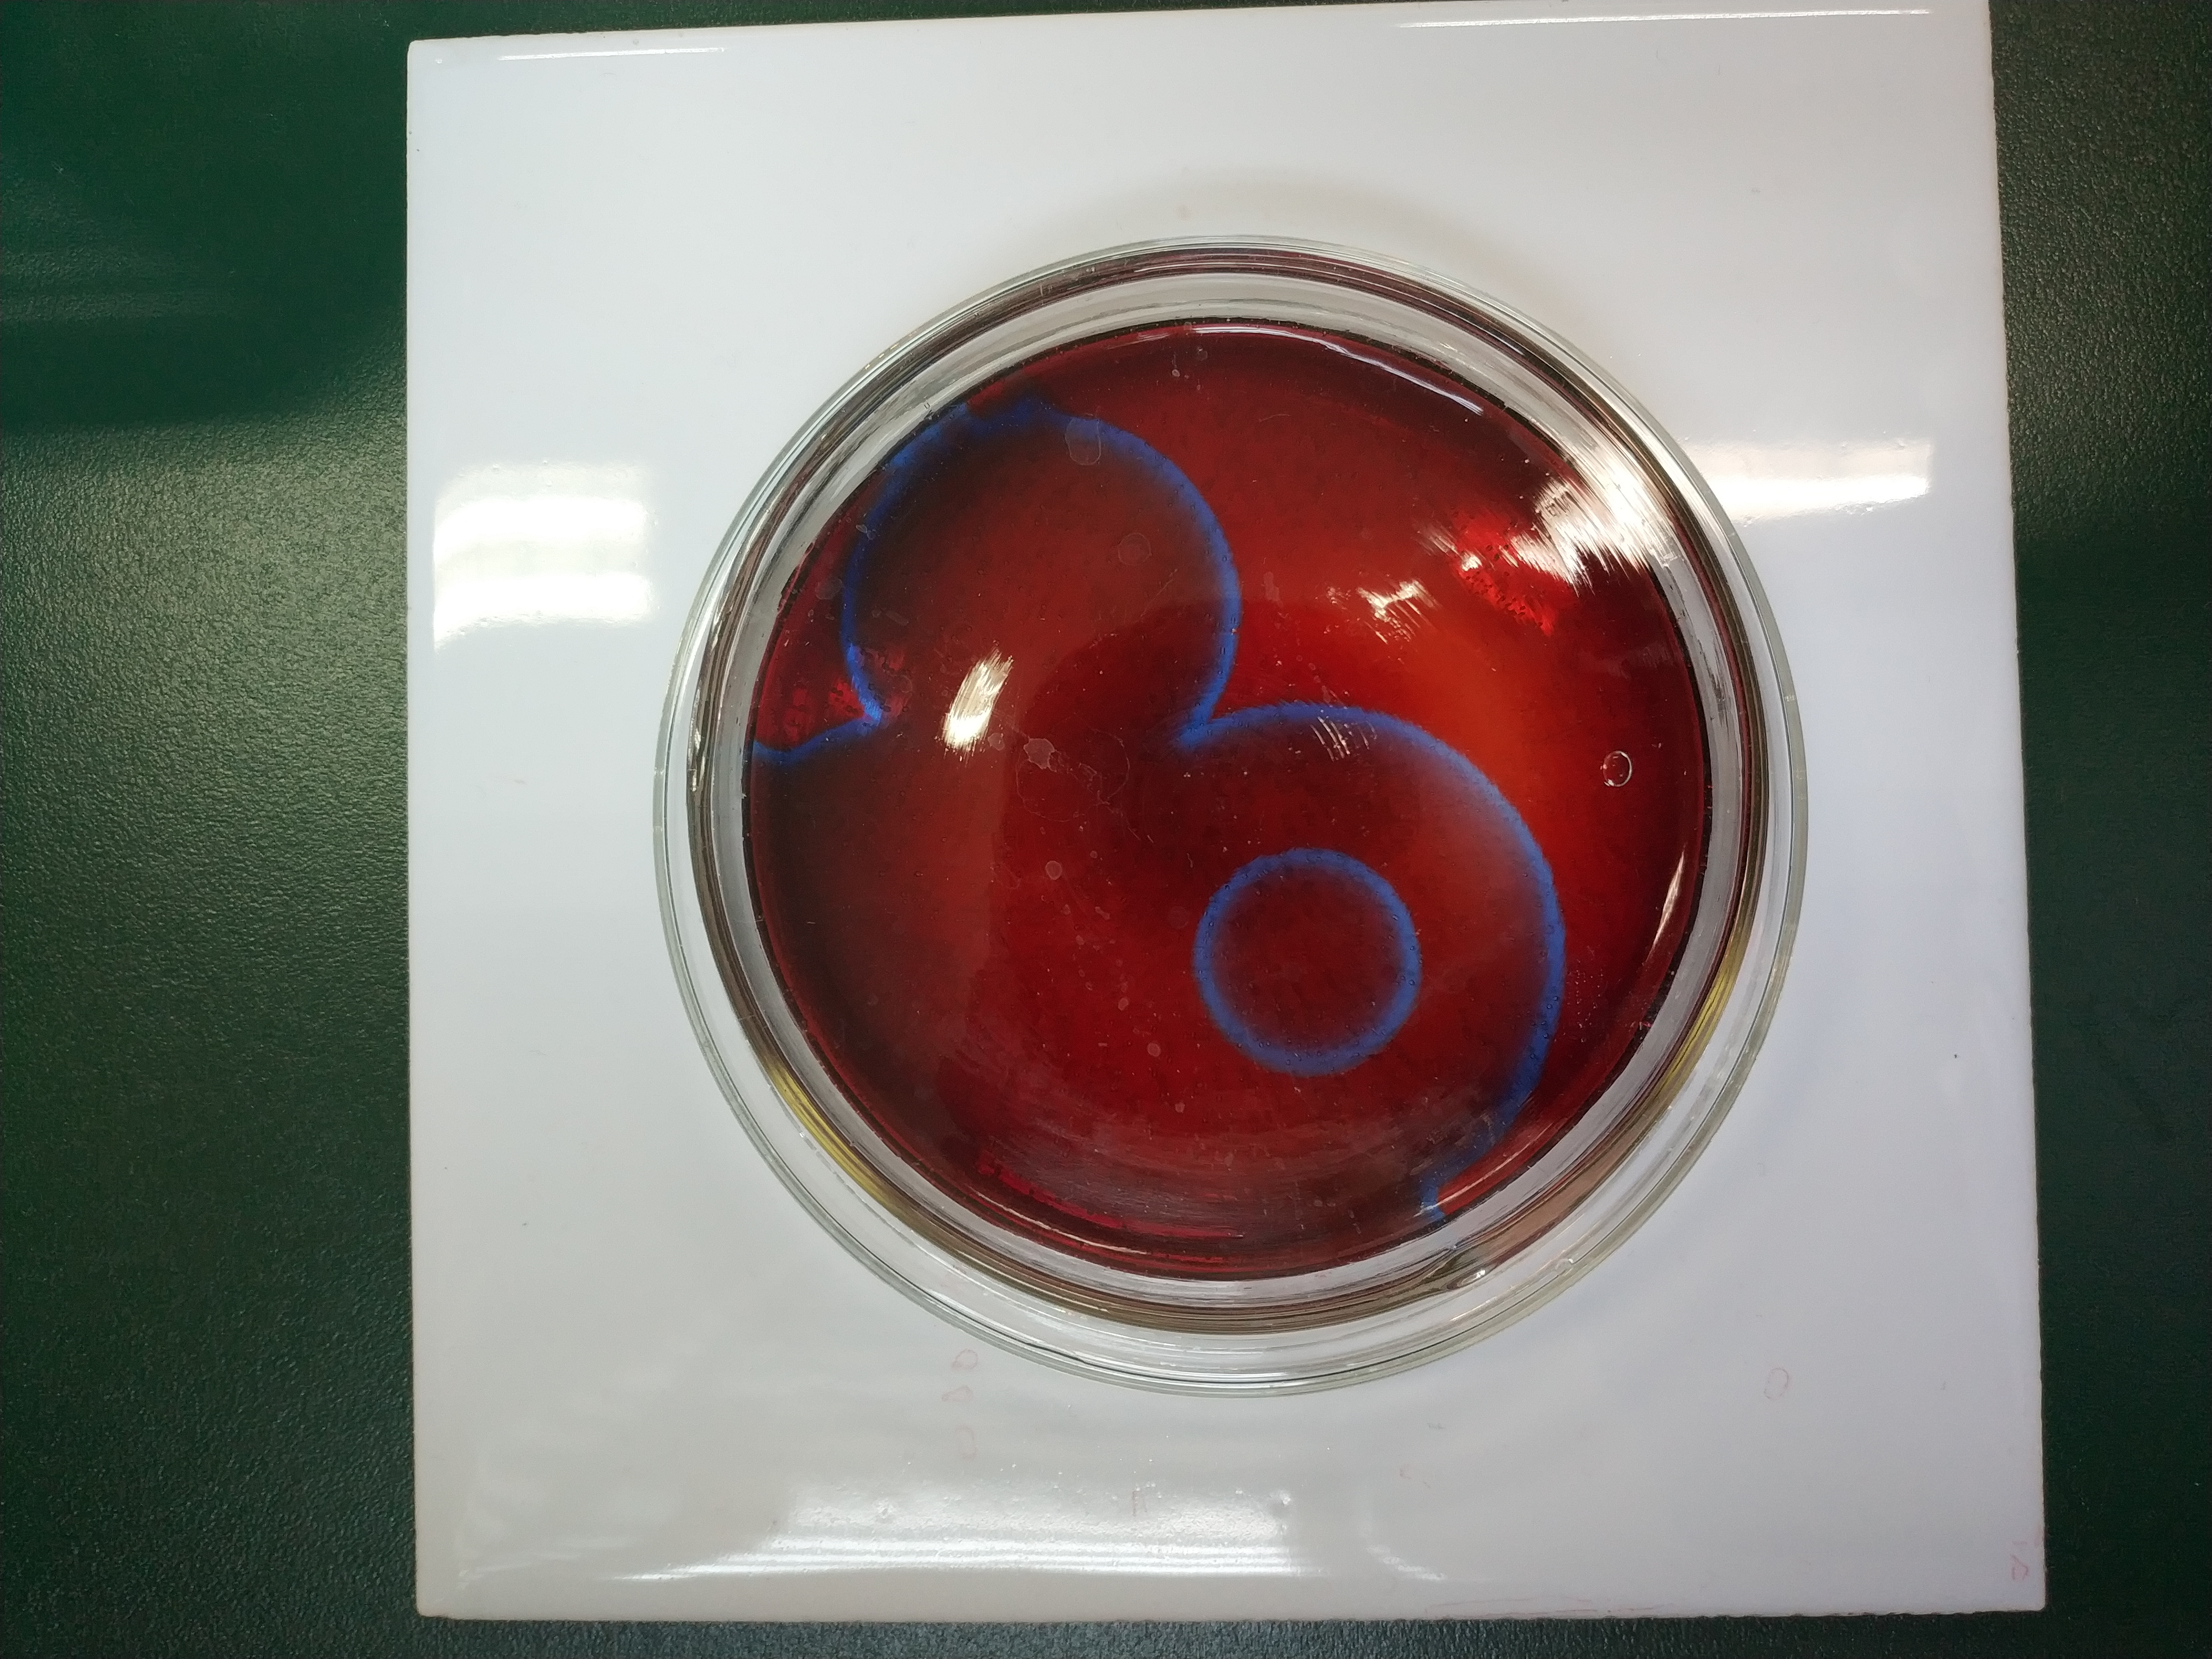
\includegraphics[width=0.30\paperwidth]{fig/circle1.jpg}\\
		\caption{同心圆实验1}
	\end{figure}
	\begin{figure}[!h]
		\centering
		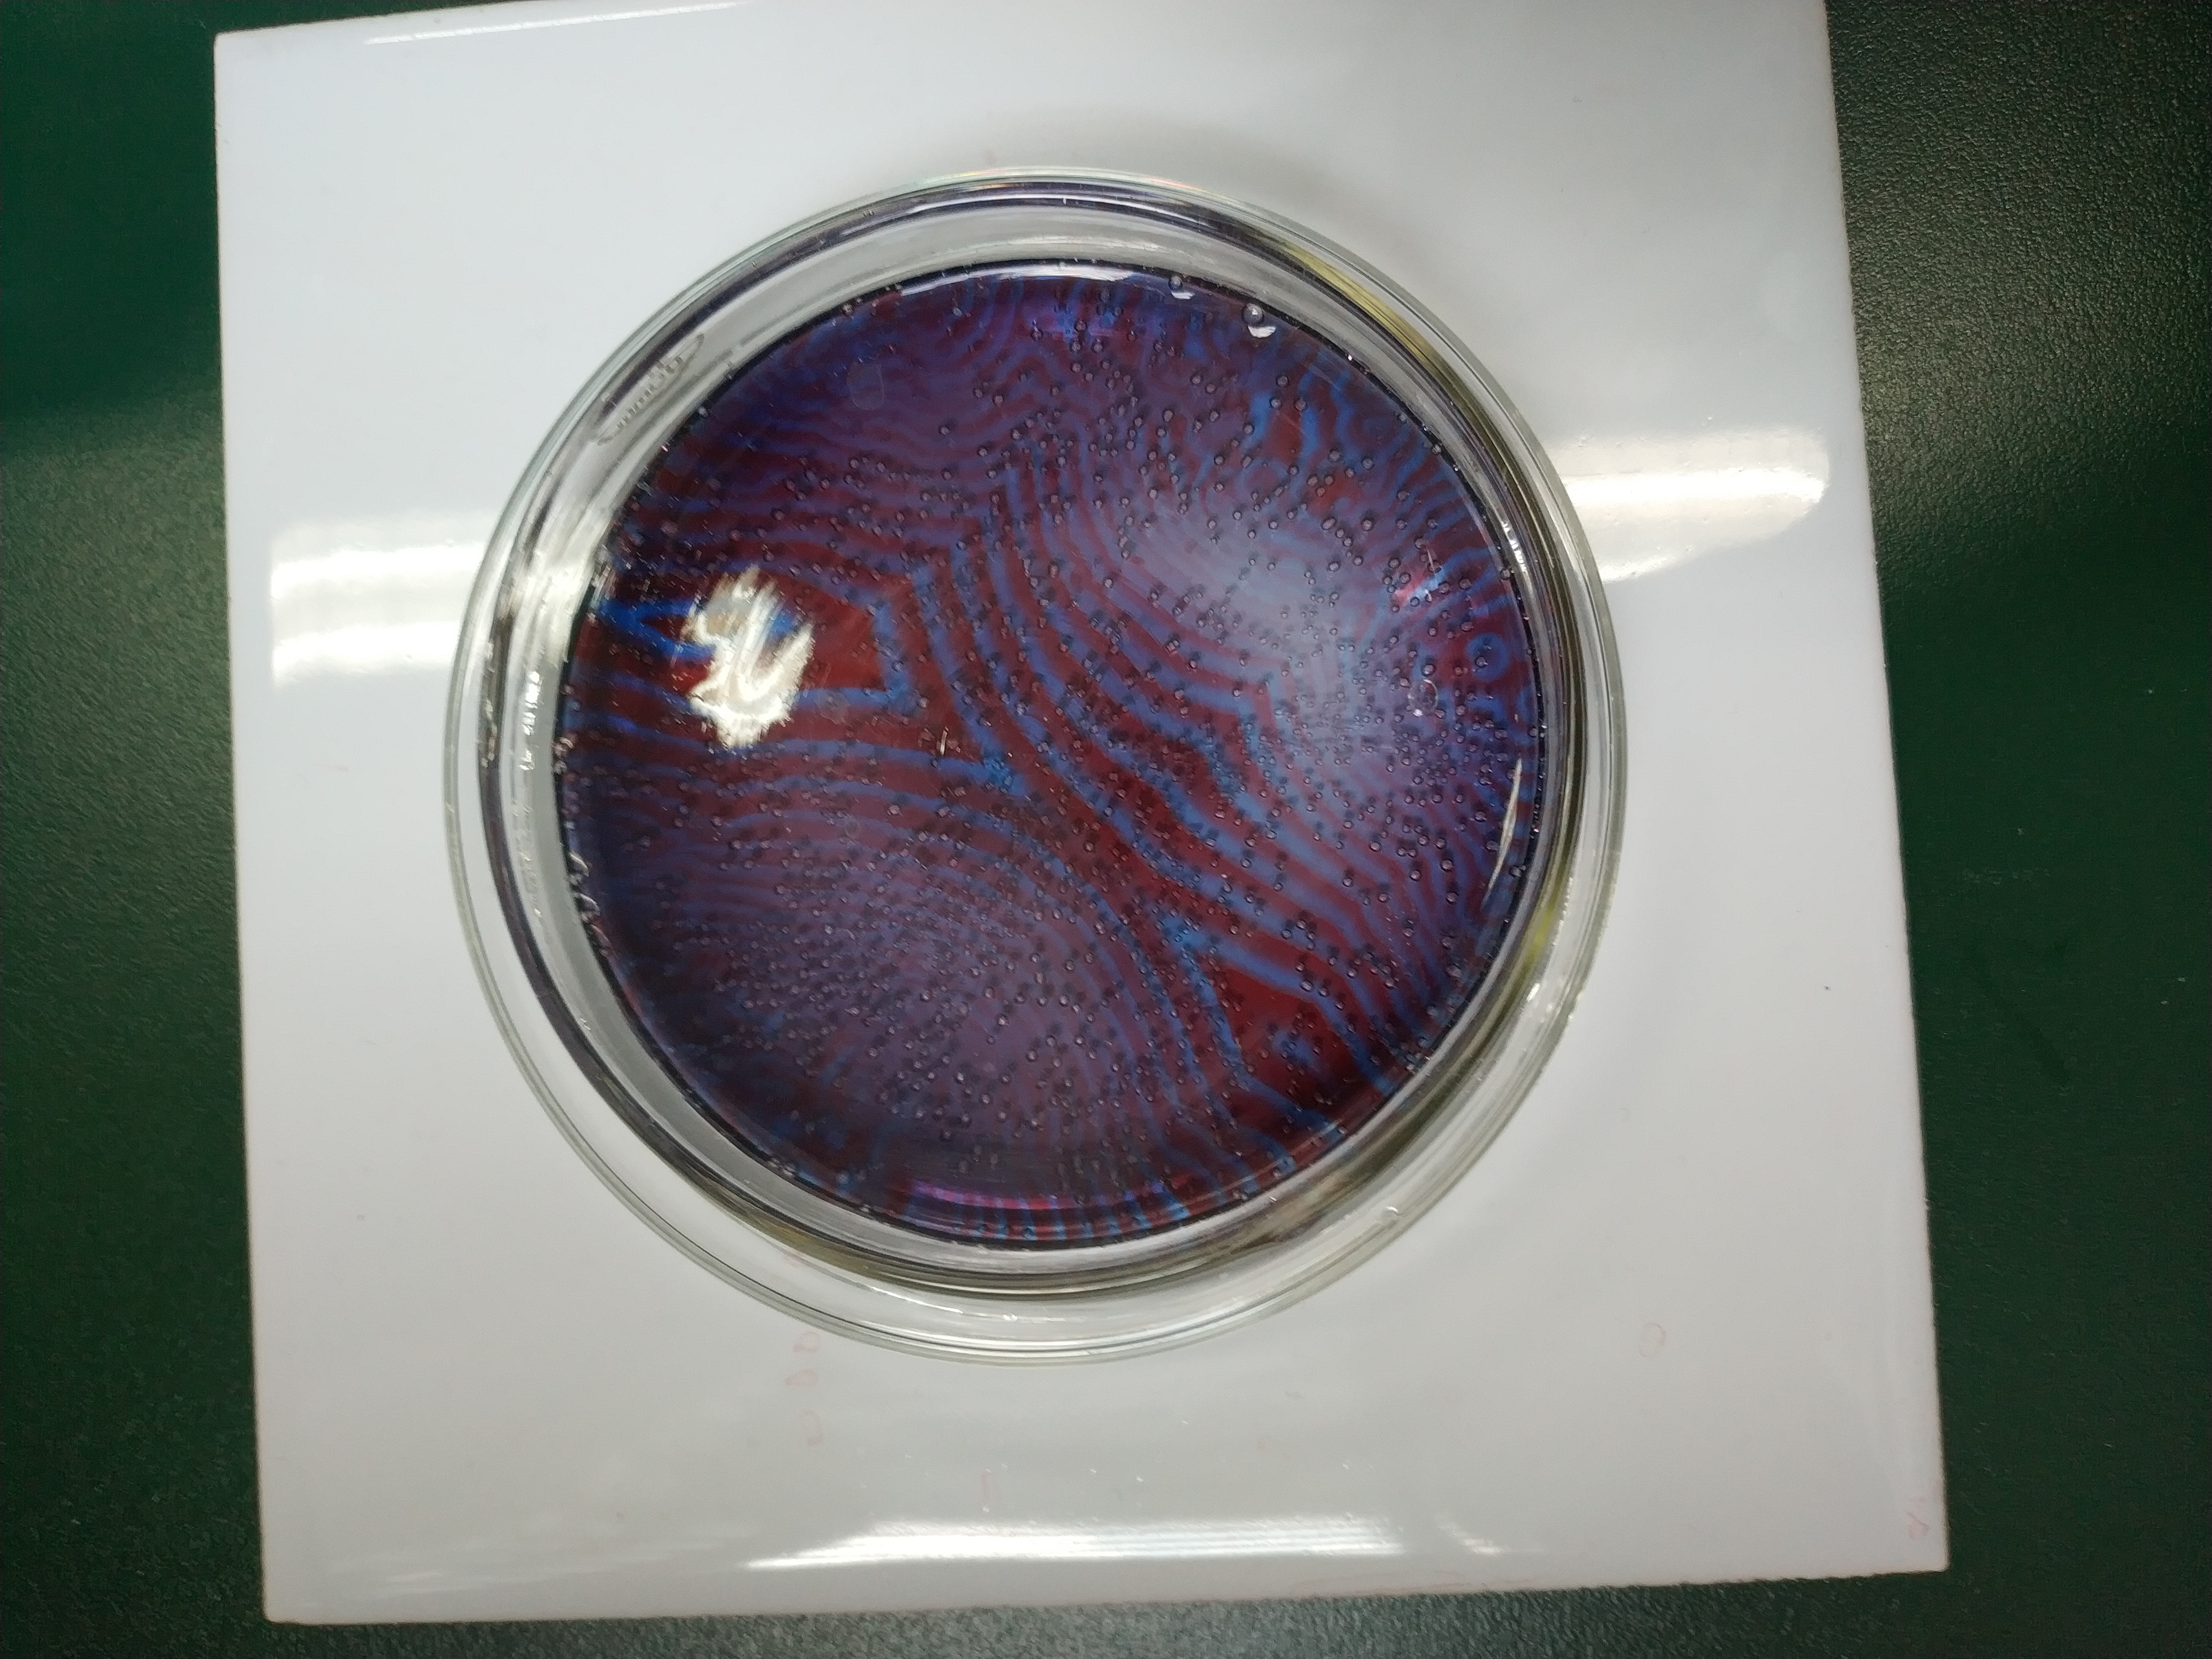
\includegraphics[width=0.30\paperwidth]{fig/circle2.jpg}\\
		\caption{同心圆实验2}
	\end{figure}
	\item 拓展实验: 测量过程中电极上会产生气泡, 在静置磁子的拓展实验中,
	实验结束时可以看到磁子上有明显的气泡. 振荡周期和振幅呈现不规则变化.
	\item 拓展实验: 亚铁灵试剂的催化作用明显强于硫酸铈铵溶液, 因此在电势测量过程中可以
	观察到在亚铁灵试剂催化下, 电势呈现振荡走低, 说明反应向一个稳态倾斜. 
	体系颜色在蓝色和紫色间周期性变化, 电势高时为蓝色, 
	电势低时为紫色. 


\end{enumerate}
\section{误差分析}
\begin{enumerate}
	\item 实验数据拟合结果中$R^{2}$极接近1, 
	因此由一次操作造成的偶然误差可以忽略. 
	\item 计算出的诱导期表观活化能为$50.65 kJ/mol$. 
	\item 恒温时间过长会导致丙二酸等溶剂挥发, 导致溶液浓度变化.
	\item 在进行不同硫酸浓度的拓展实验时, 
	可能因为前一组将催化剂类型变成了稀释10倍的亚铁灵试剂, 因此
	测得的诱导期变短, 导致实验结果有误.
\end{enumerate}
\newpage
\section{原始数据记录}
\begin{table}[!h]
	\begin{center}
		\begin{tabular}{l|l|l|l|l|l}
			\hline
			试剂&  溴酸钾&  溴化钾& 硫酸 & 硫酸铈铵 & 丙二酸\\
			\hline
			浓度$mol\cdot L^{-1}$&  &  &  &  &\\
			\hline
		 \end{tabular}
	\end{center}
\end{table}
\begin{table}[!h]
	\begin{center}
		\begin{tabular}{l|l|l|l|l|l}
			\hline
			温度/$^\circ$C&  诱导起始时间/s&  诱导终止时间/s& 诱导期t/s & $\frac{1}{t}$ & $\ln{\frac{1}{t}}$\\
			\hline
			30&  &  &  &  &\\
			\hline
			35&  &  &  &  &\\
			\hline
			40&  &  &  &  &\\
			\hline
			45&  &  &  &  &\\
			\hline
			50&  &  &  &  &\\
			\hline
		 \end{tabular}
	\end{center}
\end{table}
\begin{table}[!h]
	\begin{center}
		\begin{tabular}{l|l|l|l|l|l|l}
			\hline
			温度/$^\circ$C&  振荡周期$t_{1}$/s & $t_{2}$/s & $t_{3}$/s & $\bar{t}$/s & $\frac{1}{\bar{t}}$ & $\ln{\frac{1}{\bar{t}}}$\\
			\hline
			30&  &  &  &  &  &\\
			\hline
			35&  &  &  &  &  &\\
			\hline
			40&  &  &  &  &  &\\
			\hline
			45&  &  &  &  &  &\\
			\hline
			50&  &  &  &  &  &\\
			\hline
		 \end{tabular}
	\end{center}
\end{table}


\bibliography{ref}
\end{document}